% Options for packages loaded elsewhere
\PassOptionsToPackage{unicode}{hyperref}
\PassOptionsToPackage{hyphens}{url}
\PassOptionsToPackage{dvipsnames,svgnames,x11names}{xcolor}
%
\documentclass[
  letterpaper,
  DIV=11,
  numbers=noendperiod]{scrartcl}

\usepackage{amsmath,amssymb}
\usepackage{lmodern}
\usepackage{iftex}
\ifPDFTeX
  \usepackage[T1]{fontenc}
  \usepackage[utf8]{inputenc}
  \usepackage{textcomp} % provide euro and other symbols
\else % if luatex or xetex
  \usepackage{unicode-math}
  \defaultfontfeatures{Scale=MatchLowercase}
  \defaultfontfeatures[\rmfamily]{Ligatures=TeX,Scale=1}
\fi
% Use upquote if available, for straight quotes in verbatim environments
\IfFileExists{upquote.sty}{\usepackage{upquote}}{}
\IfFileExists{microtype.sty}{% use microtype if available
  \usepackage[]{microtype}
  \UseMicrotypeSet[protrusion]{basicmath} % disable protrusion for tt fonts
}{}
\makeatletter
\@ifundefined{KOMAClassName}{% if non-KOMA class
  \IfFileExists{parskip.sty}{%
    \usepackage{parskip}
  }{% else
    \setlength{\parindent}{0pt}
    \setlength{\parskip}{6pt plus 2pt minus 1pt}}
}{% if KOMA class
  \KOMAoptions{parskip=half}}
\makeatother
\usepackage{xcolor}
\setlength{\emergencystretch}{3em} % prevent overfull lines
\setcounter{secnumdepth}{-\maxdimen} % remove section numbering
% Make \paragraph and \subparagraph free-standing
\ifx\paragraph\undefined\else
  \let\oldparagraph\paragraph
  \renewcommand{\paragraph}[1]{\oldparagraph{#1}\mbox{}}
\fi
\ifx\subparagraph\undefined\else
  \let\oldsubparagraph\subparagraph
  \renewcommand{\subparagraph}[1]{\oldsubparagraph{#1}\mbox{}}
\fi


\providecommand{\tightlist}{%
  \setlength{\itemsep}{0pt}\setlength{\parskip}{0pt}}\usepackage{longtable,booktabs,array}
\usepackage{calc} % for calculating minipage widths
% Correct order of tables after \paragraph or \subparagraph
\usepackage{etoolbox}
\makeatletter
\patchcmd\longtable{\par}{\if@noskipsec\mbox{}\fi\par}{}{}
\makeatother
% Allow footnotes in longtable head/foot
\IfFileExists{footnotehyper.sty}{\usepackage{footnotehyper}}{\usepackage{footnote}}
\makesavenoteenv{longtable}
\usepackage{graphicx}
\makeatletter
\def\maxwidth{\ifdim\Gin@nat@width>\linewidth\linewidth\else\Gin@nat@width\fi}
\def\maxheight{\ifdim\Gin@nat@height>\textheight\textheight\else\Gin@nat@height\fi}
\makeatother
% Scale images if necessary, so that they will not overflow the page
% margins by default, and it is still possible to overwrite the defaults
% using explicit options in \includegraphics[width, height, ...]{}
\setkeys{Gin}{width=\maxwidth,height=\maxheight,keepaspectratio}
% Set default figure placement to htbp
\makeatletter
\def\fps@figure{htbp}
\makeatother

\KOMAoption{captions}{tableheading}
\makeatletter
\makeatother
\makeatletter
\makeatother
\makeatletter
\@ifpackageloaded{caption}{}{\usepackage{caption}}
\AtBeginDocument{%
\ifdefined\contentsname
  \renewcommand*\contentsname{Table of contents}
\else
  \newcommand\contentsname{Table of contents}
\fi
\ifdefined\listfigurename
  \renewcommand*\listfigurename{List of Figures}
\else
  \newcommand\listfigurename{List of Figures}
\fi
\ifdefined\listtablename
  \renewcommand*\listtablename{List of Tables}
\else
  \newcommand\listtablename{List of Tables}
\fi
\ifdefined\figurename
  \renewcommand*\figurename{Figure}
\else
  \newcommand\figurename{Figure}
\fi
\ifdefined\tablename
  \renewcommand*\tablename{Table}
\else
  \newcommand\tablename{Table}
\fi
}
\@ifpackageloaded{float}{}{\usepackage{float}}
\floatstyle{ruled}
\@ifundefined{c@chapter}{\newfloat{codelisting}{h}{lop}}{\newfloat{codelisting}{h}{lop}[chapter]}
\floatname{codelisting}{Listing}
\newcommand*\listoflistings{\listof{codelisting}{List of Listings}}
\makeatother
\makeatletter
\@ifpackageloaded{caption}{}{\usepackage{caption}}
\@ifpackageloaded{subcaption}{}{\usepackage{subcaption}}
\makeatother
\makeatletter
\@ifpackageloaded{tcolorbox}{}{\usepackage[many]{tcolorbox}}
\makeatother
\makeatletter
\@ifundefined{shadecolor}{\definecolor{shadecolor}{rgb}{.97, .97, .97}}
\makeatother
\makeatletter
\makeatother
\ifLuaTeX
  \usepackage{selnolig}  % disable illegal ligatures
\fi
\usepackage[]{biblatex}
\IfFileExists{bookmark.sty}{\usepackage{bookmark}}{\usepackage{hyperref}}
\IfFileExists{xurl.sty}{\usepackage{xurl}}{} % add URL line breaks if available
\urlstyle{same} % disable monospaced font for URLs
\hypersetup{
  pdftitle={人工土的制备},
  pdfauthor={舒子豪},
  colorlinks=true,
  linkcolor={blue},
  filecolor={Maroon},
  citecolor={Blue},
  urlcolor={Blue},
  pdfcreator={LaTeX via pandoc}}

\title{人工土的制备}
\usepackage{etoolbox}
\makeatletter
\providecommand{\subtitle}[1]{% add subtitle to \maketitle
  \apptocmd{\@title}{\par {\large #1 \par}}{}{}
}
\makeatother
\subtitle{按照一定比例混合针铁矿、高岭土及石英砂得到人工土}
\author{舒子豪}
\date{9/26/22}

\begin{document}
\maketitle
\ifdefined\Shaded\renewenvironment{Shaded}{\begin{tcolorbox}[frame hidden, enhanced, interior hidden, boxrule=0pt, breakable, borderline west={3pt}{0pt}{shadecolor}, sharp corners]}{\end{tcolorbox}}\fi

\hypertarget{ux7406ux8bbaux57faux7840}{%
\section{理论基础}\label{ux7406ux8bbaux57faux7840}}

铁在地壳内的数量仅次于\textbf{氧}、\textbf{硅}和\textbf{铝},位居第四,在地壳中的含量丰富且氧化还原性质活跃。土壤中的铁几乎以\textbf{氧化铁}的形态存在,成土过程中母质风化的产物经过再积淀是土壤中氧化铁的主要成因,矿物中的铁在风化作用下游离在硅酸盐外,形成了氧化铁\footnote{王璐莹,秦雷,吕宪国,姜明,邹元春.
  \href{https://kns.cnki.net/kcms/detail/detail.aspx?dbcode=CJFD\&dbname=CJFDLAST2018\&filename=TRXB201805001\&uniplatform=NZKPT\&v=S6JMDESWy88roKn6cxwfV1jDuxaPt_WUctWqUfpeOvB47_1Lnx2A4hxIoPX5gcWI}{铁促进土壤有机碳累积作用研究进展}{[}J{]}.土壤学报,2018,55(05):1041-1050.}。

土壤中常见的氧化铁为\textbf{赤铁矿(Hematite,α-Fe2O3)}、\textbf{磁赤铁矿(Maghemite,γ-Fe2O3)}、\textbf{针铁矿(Goethite,α-FeO(OH))}、\textbf{纤铁矿(Lepidocrocite,γ-FeO(OH))}、\textbf{水铁矿}和\textbf{氢氧化铁凝胶}。

\textbf{土壤中氧化铁的主要存在形态包括:}

\begin{itemize}
\item
  游离态氧化铁(Fed)是指土壤中排除在层状硅酸盐组成部分之外的铁,主要是土壤黏粒中的铁氧化物和水化合物,也可以定义为可以用连二亚硫酸钠-柠檬酸钠-重碳酸钠(DCB)法提取的氧化铁。土壤中或土壤粘粒中的游离态铁氧化物在全铁(FeT)中所占的百分数即为\textbf{铁的游离度(100
  × Fed/FeT)},对反映土壤风华程度具有重要意义。
\item
  无定形态氧化铁(Feo)是指能用\textbf{草酸铵}提取的氧化铁,是游离态氧化铁中的一部分,活性较高,比表面积较大,不发生X射线衍射的水合氧化铁。无定形铁在游离态铁中所占的百分比叫做\textbf{氧化铁的活化度(100
  ×
  Feo/Fed)},可判定土壤的发生特征和土类,反映某些成土环境对土壤发生的影响。\textbf{(1-100
  ×
  Feo/Fed)}表示氧化铁的老化程度。游离氧化铁与无定形氧化铁(Feo)的差值为晶质氧化铁。
\item
  络合态氧化铁(Fep)是指能够与土壤腐殖质形成络合物,即能被\textbf{焦磷酸钠}提取的那部分氧化铁,属于无定形物质,但是由于不能完全被\textbf{草酸铵缓冲溶液}提取,因此,并不完全包含于无定形铁中。络合态铁占游离态铁的百分比为铁的络合度(100
  ×
  Fep/Fed),土壤络合铁的含量和络合度与有机质含量正相关,是铁离子在土壤中迁移转化的主要原因之一。
\end{itemize}

针铁矿广泛存在于土壤中(热带和亚热带土壤含量较高),虽然在数量上是土壤的次要成分,但是其本身的性质及对土壤反应所起的作用和对层状矿物有重要的影响。土壤中针铁矿以单独的晶体、凝胶态、斑状、胶膜等形式存在,\textbf{人工合成的针铁矿以晶体形式存在,其电荷零点(ZPC)较高},但同土壤中的针铁矿一样其表面积较大、表面活性官能团较多、电荷的可变性墙,对土壤的物理化学特性,尤其是营养元素的吸附、迁移有及其重要的作用。相对于天然形成的针铁矿,合成针铁矿具有纯度高、方便易得、可重复制备等优点\footnote{Rakhsh
  F, Golchin A, Al Agha A B, et al.~\href{}{Mineralization of organic
  carbon and formation of microbial biomass in soil: Effects of clay
  content and composition and the mechanisms involved}{[}J{]}. Soil
  Biology and Biochemistry, 2020, 151: 108036.}。

自1976年Atkinson等人用合成的针铁矿进行吸附实验研究之后,相继有很多研究学者对合成针铁矿进行了研究探索。主要合成方法有水热法和水解中和法。水热法在高温高压的反应釜中进行,反应时间短但反应条件不易实现,所以使用最对的是水解中和法\footnote{刘永红,叶发兵,岳霞丽,董元彦.
  \href{https://kns.cnki.net/kcms/detail/detail.aspx?dbcode=CJFD\&dbname=CJFD2006\&filename=HBHG200607003\&uniplatform=NZKPT\&v=lAapXeiCwvyIGjrWJHKZjrtB_0ef5XTFpkSGFn65obDsNFp7-P8iz6zbinJPP1H5}{铁氧化物的合成及其表征}{[}J{]}.化学与生物工程,2006(07):10-12.}。

\textbf{水解中和法制备条件对合成针铁矿的影响:}

\begin{enumerate}
\def\labelenumi{\arabic{enumi}.}
\item
  在制备针铁矿的实验过程中,酸性条件和常温磁力搅拌都不利于前驱体转化为针铁矿,不利于形成针铁矿结晶,老化时间对针铁矿结晶程度和晶体生长有一定影响。优化的针铁矿制备条件为:碱性条件下70℃老化48
  h以上。
\item
  矿化剂混合方式不会影响针铁矿物相的形成,但对针铁矿的结晶形貌、粒径大小、团聚程度和比表面积产生一定影响。优化条件下迅速混合矿化剂,可制得结晶程度好,粒度分布均匀,比表面积较大得较为均一的雪花针铁矿;逐滴滴加矿化剂可制得结晶程度好,较均匀分布得条柱状针铁矿\footnote{吴思源,练有为,郑红,蔡鹏,濮玉兵.
    \href{https://kns.cnki.net/kcms/detail/detail.aspx?dbcode=CJFD\&dbname=CJFD2012\&filename=HJHX201210024\&uniplatform=NZKPT\&v=6MaQ-CmnMRBerybdZXrj-fwGF93WX3xs4k9-cDGherPIfJnJBK00SU6d2NWDliwb}{制备条件对合成针铁矿的影响}{[}J{]}.环境化学,2012,31(10):1625-1630.}。
\end{enumerate}

\hypertarget{ux6750ux6599ux51c6ux5907}{%
\section{材料准备}\label{ux6750ux6599ux51c6ux5907}}

\begin{itemize}
\item
  石英砂
\item
  九水硝酸铁(Fe(NO3)3·9H2O)又名硝酸高铁浅紫色或灰白色单斜晶体,易潮解。1
  M的九水硝酸铁溶液配制:称取40.4 g九水硝酸铁溶解于100
  ml蒸馏水中摇匀,备用。
\item
  氢氧化钾(KOH)
\item
  氯化钙(CaCl2)
\item
  高岭土(Al2O3·2Si2O2·2H2O2)
\end{itemize}

\hypertarget{ux5236ux5907ux8fc7ux7a0b}{%
\section{制备过程}\label{ux5236ux5907ux8fc7ux7a0b}}

\begin{itemize}
\item
  石英砂的制备将不同粒径的石英砂分别过2 mm和0.05 mm筛,取留在0.05
  mm筛上的石英砂。水洗后置于马弗炉中在550℃下灼烧两次,每次4
  h。冷却至室温后用2 M
  HCl清洗石英砂脱除碳酸盐,用蒸馏水洗涤后在105℃下烘干备用\footnote{Rakhsh
    F, Golchin A, Al Agha A B, et
    al.~\href{https://doi.org/10.1016/j.geoderma.2017.07.010}{Effects of
    exchangeable cations, mineralogy and clay content on the
    mineralization of plant residue carbon}{[}J{]}. Geoderma, 2017, 307:
    150-158.}。
\item
  针铁矿的制备用180 ml 5 M KOH 与100 ml 1 M Fe(NO3)3·9H2O中和,然后用2 L
  蒸馏水稀释并在70℃下密闭保存60
  h,最后洗涤产物去除OH-、NO3-,冷冻干燥后备用\footnote{Schwertmann U,
    Cornell R M.
    \href{https://doi.org/10.1180/claymin.1992.027.3.14}{Iron oxides in
    the laboratory: preparation and characterization}{[}M{]}. John Wiley
    \& Sons, 2008.}。
\end{itemize}

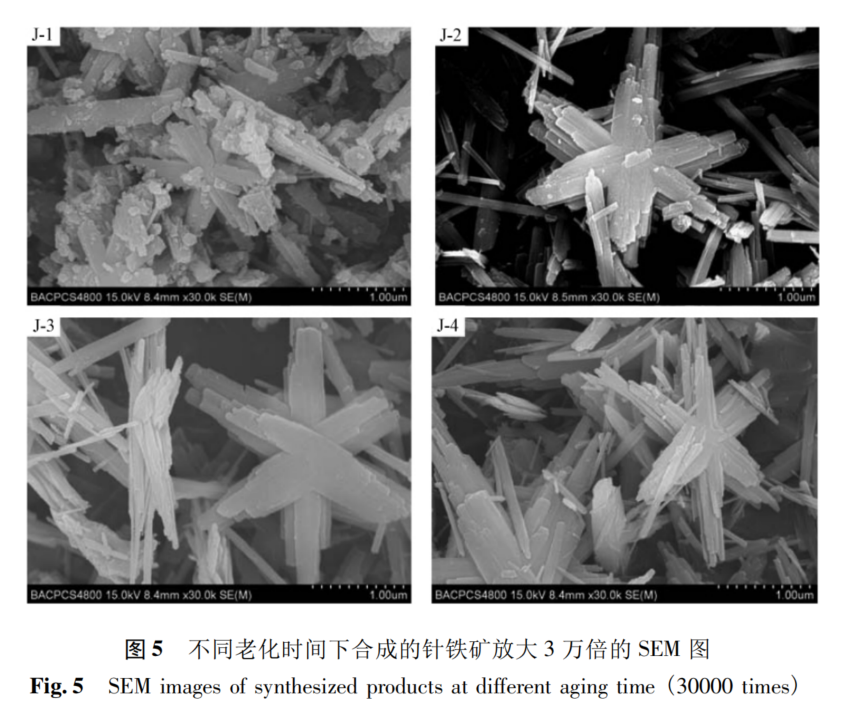
\includegraphics{针铁矿的制备.png}

\begin{itemize}
\item
  高岭土的制备水洗高岭土粉末,去除杂质,提高纯度,得到\textless2
  μm的细组分,冷冻干燥后备用。
\item
  粘土的制备将高岭土与针铁矿以10:1 (w:w)混合,加入0.01 M
  CaCl2(10:1,v:w)制备悬浮液。将悬浮液搅拌24 h,在5500 g下离心10
  min,倒去上清液,将土壤在脱盐水中重悬浮后再次离心10
  min,重复重悬浮过程,直到上清液EC\textless100
  μS/cm,得到的土壤冷冻干燥后过210 μm筛备用\footnote{Rakhsh F, Golchin
    A, Al Agha A B, et
    al.~\href{https://doi.org/10.1016/j.soilbio.2020.108036}{Mineralization
    of organic carbon and formation of microbial biomass in soil:
    Effects of clay content and composition and the mechanisms
    involved}{[}J{]}. Soil Biology and Biochemistry, 2020, 151: 108036.}\footnote{Saidy
    A R, Smernik R J, Baldock J A, et
    al.~\href{https://doi.org/10.1016/j.geoderma.2011.12.030}{Effects of
    clay mineralogy and hydrous iron oxides on labile organic carbon
    stabilisation}{[}J{]}. Geoderma, 2012, 173: 104-110.}。
\item
  人工土壤的制备将石英砂与黏土按一定比例(45\%)混合,测定持水能力,并在高压灭菌锅中120℃下湿蒸3次,每次2
  h,去除土壤微生物\footnote{Cai Y, Ma T, Wang Y, et
    al.~\href{https://doi.org/10.1016/j.geoderma.2021.115562}{Assessing
    the accumulation efficiency of various microbial carbon components
    in soils of different minerals}{[}J{]}. Geoderma, 2022, 407: 115562.}。
\end{itemize}


\printbibliography[title=参考资料]


\end{document}
